\documentclass{beamer}

\mode<presentation> {

\usetheme{metropolis} 

%\usetheme[subsectionpage=progressbar]{metropolis}

%\setbeamertemplate{footline} % To remove the footer line in all slides uncomment this line
\setbeamertemplate{footline}[page number] % To replace the footer line in all slides with a simple slide count uncomment this line

%\setbeamertemplate{navigation symbols}{} % To remove the navigation symbols from the bottom of all slides uncomment this line
}

\usepackage{graphicx} % Allows including images
\usepackage{booktabs}

\usepackage{gensymb} % Allows the use of \toprule, \midrule and \bottomrule in tables
\usepackage{caption}   % For caption under images
\captionsetup[figure]{
    position=below,
}

\title[Design Project]{Point Cloud Generation} 

\author{Mohit Rajan\newline Nandini Menon\newline Pooja Sivakumar   \newline Sanjay Govind} 
\institute[FISAT] % Your institution as it will appear on the bottom of every slide, may be shorthand to save space
{
FISAT \\ % Your institution for the title page
\medskip
%\textit{} % Your email address
}


\begin{document}

\begin{frame}
\titlepage % Print the title page as the first slide
\end{frame}

\begin{frame}{Table of Contents}
\tableofcontents
\newpage
\end{frame}

%----------------------------------------------------------------------------------------
%	PRESENTATION SLIDES
%----------------------------------------------------------------------------------------

\section{Abstract} % Sections can be created in order to organize your presentation into discrete blocks, all sections and subsections are automatically printed in the table of contents as an overview of the talk
%------------------------------------------------

\begin{frame}
\frametitle{Abstract}
 This project aims at building a robot that visualizes its surroundings  by using  Arduino to control the hardware  and PCL  for  visualizing the data.
%\par This project is generate a point cloud and visualise it . A robotic arm with a ultrasonic sensor at end effector sweeps  $360\degree$  and  determines the distances from obstacles present nearby.Using the data a point cloud is generated and visualised to create a 3-D representation of the obstacles.
\end{frame}

%------------------------------------------------
\section{Objective}
\begin{frame}
\begin{itemize}
%\item To visualize a point cloud
\item The objective of the project is to retrive data from surroundings and to create and visualize a Point Cloud.
\end{itemize}
\end{frame}



\section{Introduction}

\begin{frame}{Robotic Arm}
\begin{itemize}
\item Mechanical Arm, which is programmable
\item Similar functions to a human arm
\item Links connected by joints allowing either rotational motion or translational displacement
\item End of the manipulator called End Effector
\end{itemize} 
\end{frame}

\begin{frame}{uArm}
\begin{itemize}
\item Open Source robotic arm that can be assembled and controlled
\item Manufactured by UFACTORY
\end{itemize}
\begin{figure}
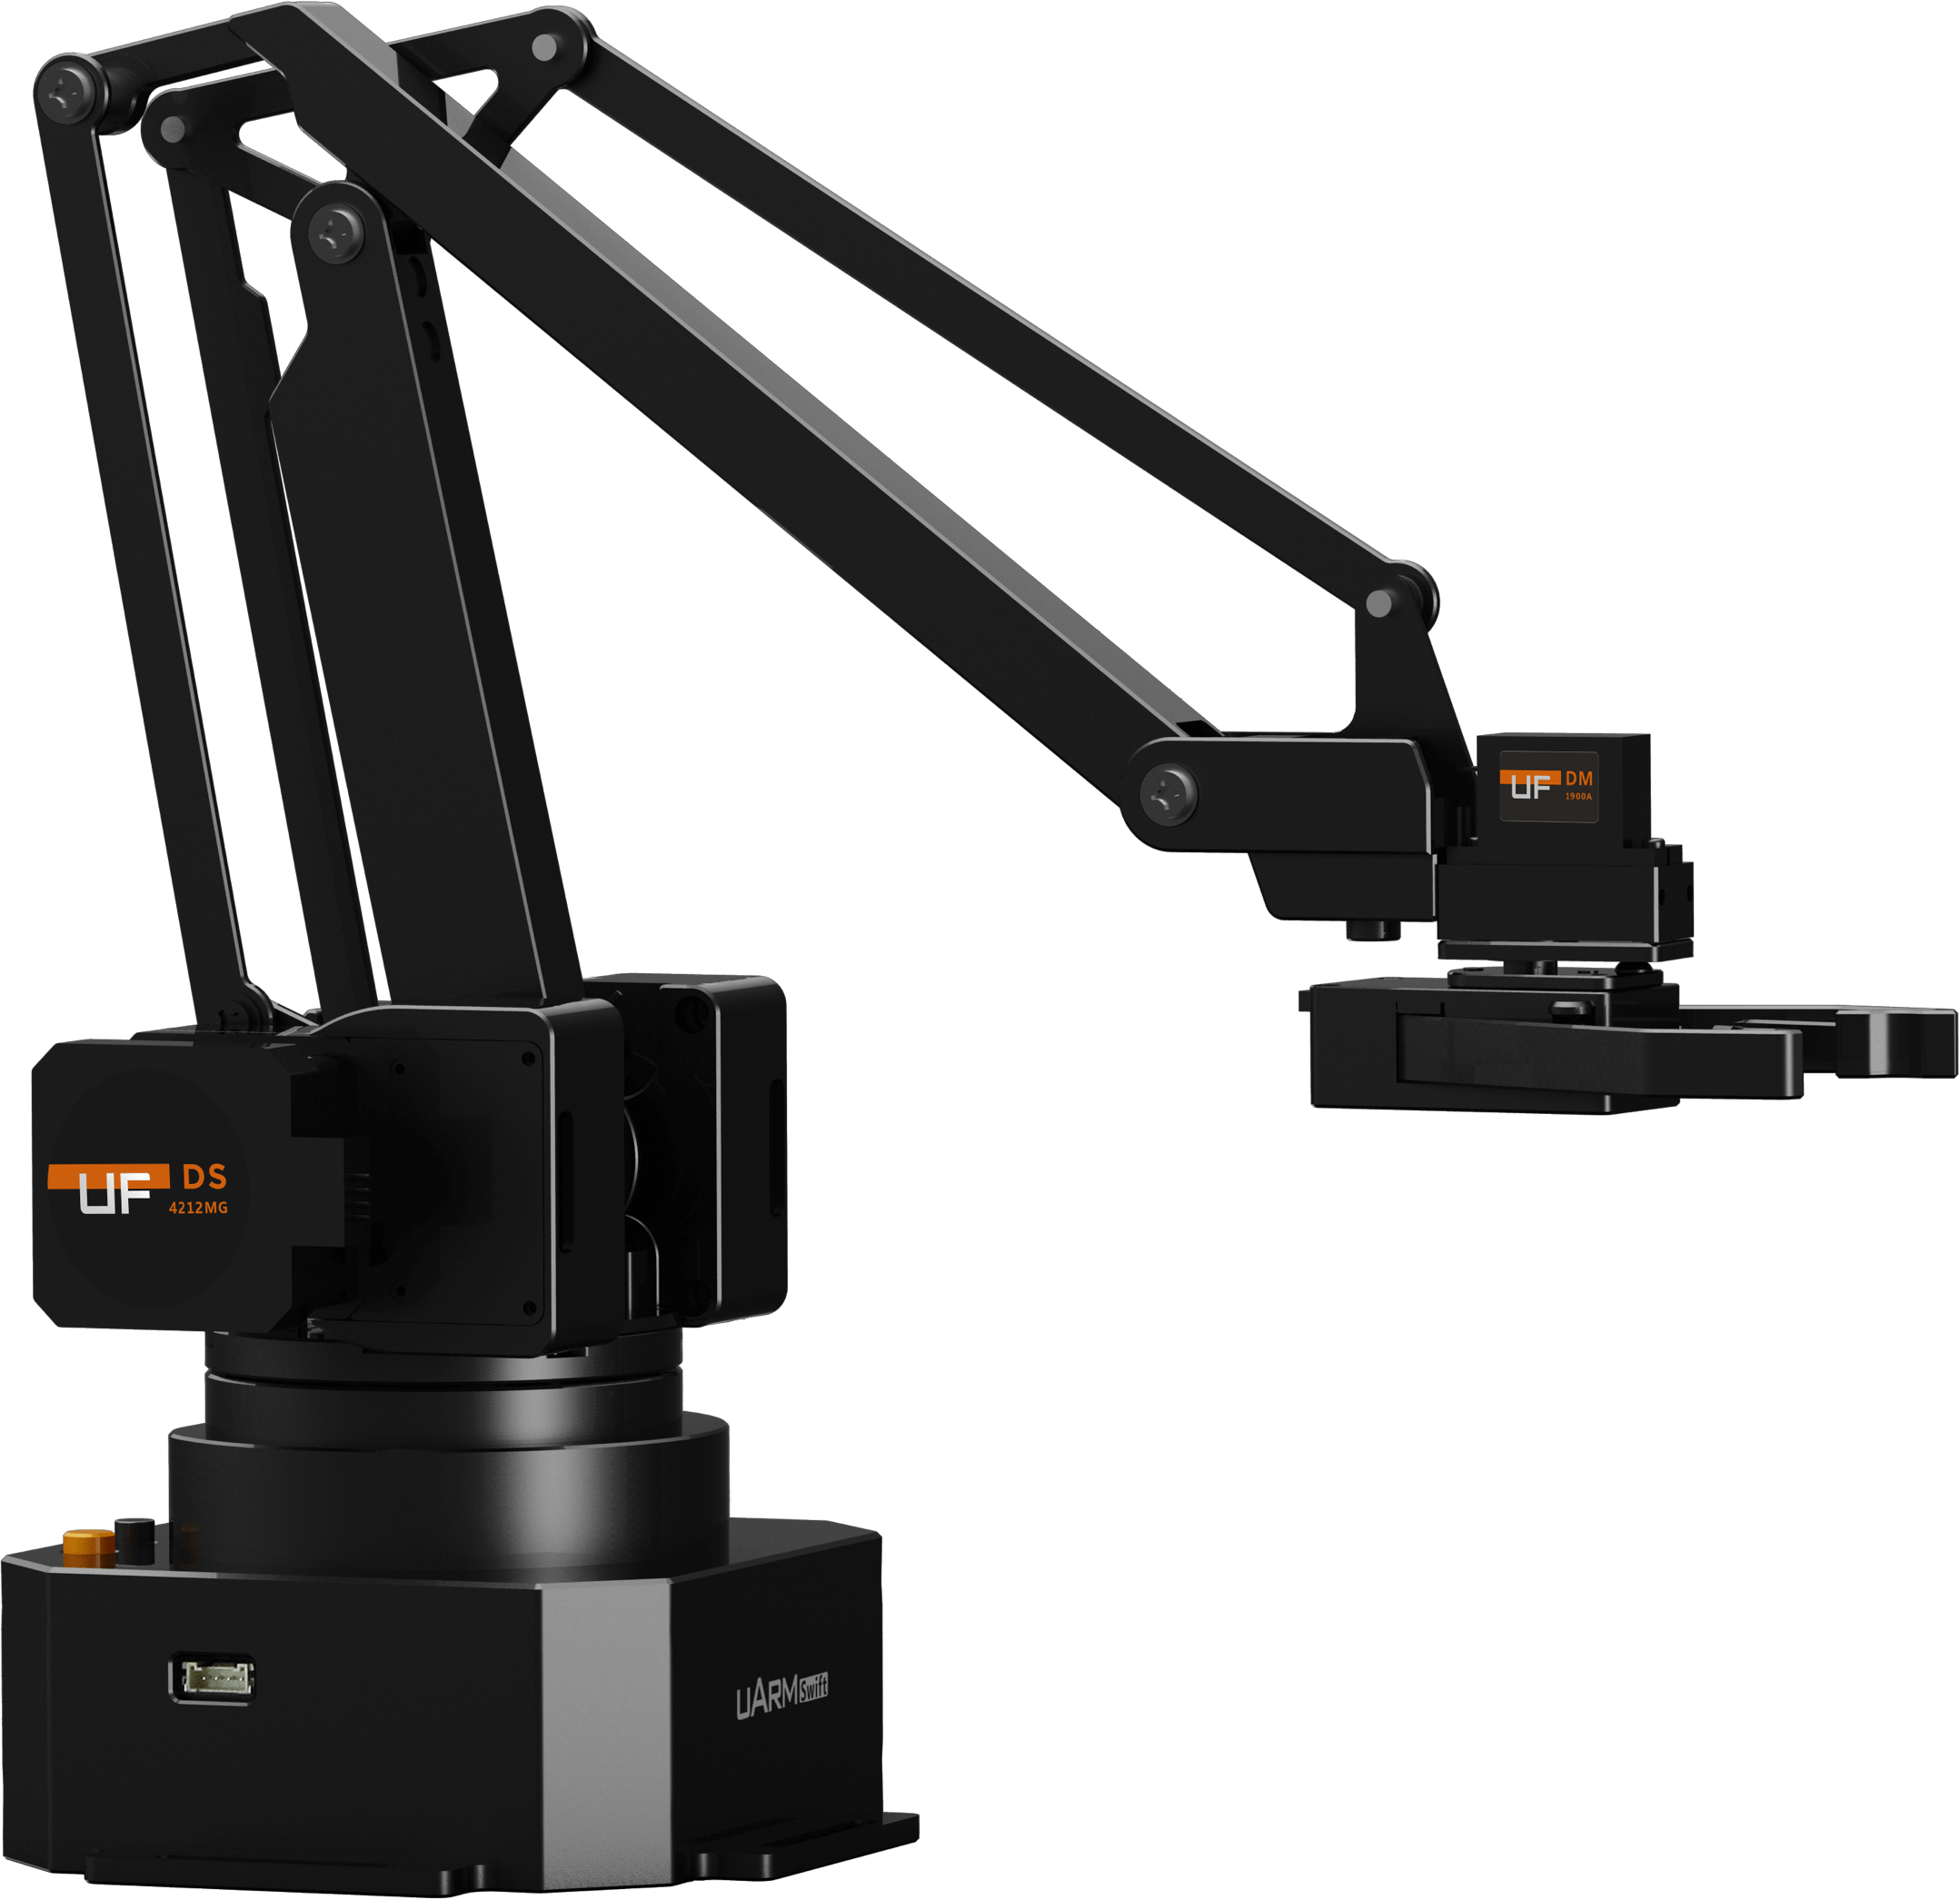
\includegraphics[scale=0.075]{uarm.png}
\end{figure}
\end{frame}

\begin{frame}[fragile]
\frametitle{Point Cloud}
\begin{itemize}
%\item Point clouds are a collection of points that represent a 3D shape or feature. Each point has its own set of X, Y and Z coordinates and in some cases additional attributes. We can think about a point cloud as a collection of multiple points
\item Huge number of tiny data points existing in three dimensions
\item Used to represent a 3-D shape or feature
\end{itemize}
\begin{figure}
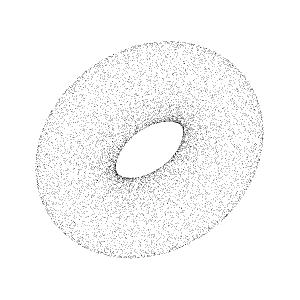
\includegraphics[width=4cm]{pc.png}
\end{figure}
\end{frame}

\begin{frame}[fragile]{LIDAR}
\begin{itemize}
\item Stands for LIght Detection And Ranging.
\item Remote Sensing Method.
\item Uses light in the form of a pulsed laser to measure ranges.
%ranges - variable distances
\item These light pulses along with other data generate precise 3-D information about the shape of the earth and it's surface characteristics.
\end{itemize}
\end{frame}

%\begin{frame}[fragile]
%\frametitle{Introduction}
%\begin{itemize}
%\item A two-joint robot with an ultrasonic sensor at end effector sweeps $360\degree$
%\item The sensor detects the distance from the obstacles in front of it by sending a sound wave and calculating how much time it takes to be reflected back
%\item Using this distance, we calculate the x, y and z coordinates.
%\item The coordinates are compiled and stored as point cloud data.
%\item Points are then plotted and visualized.
%\end{itemize}
%\end{frame}

\section{Proposed Work}
\begin{frame}
\frametitle{Proposed Work}
\begin{itemize}
\item The proposed work is to create a robot which can detect nearby objects and create a digital image of the same. 
\item The robot scans it's surroundings using HC-SR04 sensor, the distance is calculated.
\item A python script parses this data and finds the values of x, y and z.
\item This is then stored in a point cloud data file. We expect to plot these points and visualize it. 
\end{itemize}
\end{frame}

\section{Design}
\begin{frame}
\frametitle{Design}
\subsection{Hardware}
\begin{figure}
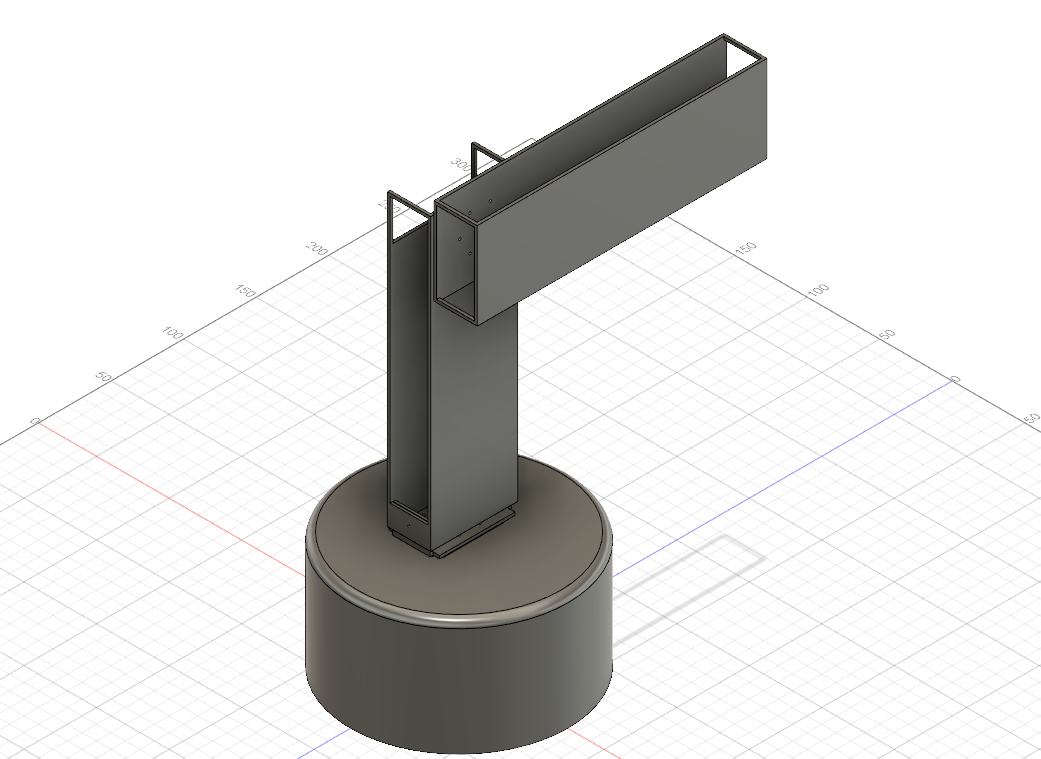
\includegraphics[scale=0.25]{hardware.png}

\end{figure}

\end{frame}

%\begin{frame}[fragile]
%\frametitle {Design}
%\subsection{Circuit design}
%\textbf{Circuit design}
%\begin{itemize}

%\item The two servo   motor's and the ultrasonic sensor are controlled by the Arduino
%\item Servo motors are used to get precise movement
%\item Connections are as shown in figure
%\end{itemize}

%\textbf{$360\degree$ Servo Motor}
%\begin{itemsize}
%\item   Since we require a $360\degree$ rotation for the base ,\textbf{V3003}, which is a $360\degree$ continous servo ,is sused as base motor.
%\item  Operating speed at no load is 0.2sec/$60\degree$ at 4.8V \newline
%0.18sec/$60\degree$ at 6V.
%\end{itemsize}



%\begin{figure}
%\includegraphics[width=5cm]{design2.png}
%\end{figure}


%\end{frame}



\begin{frame}
\begin{figure}
\frametitle{Circuit Design}
\includegraphics[scale=0.4]{design2.png}
\end{figure}
\end{frame}



\section{Completed Tasks}
 \begin{frame}
 \frametitle{Completed tasks}
 \subsection{Task 1:To  learn basics of  robotic arm manipulation}
 \textbf{Task 1: To  learn basics of robotic arm manipulation}
 \begin{itemize}
 \item Familiarised with the parts of the arm.
 \item  Learnt basic foward and inverse kinematics.
 \item  Graphical and Jacobian methods were introspected.
 \end{itemize}

\end{frame}

\begin{frame}[fragile]
\frametitle{Completed tasks}
 \subsection{Task 2:Given end effector co-ordinates, to find the joint angles}
 \textbf{Task 2: Given end effector co-ordinates, to find joint angles}
 \begin{itemize}
 \item Given a two-joint robotic arm, with base rotation of $360\degree$ and other joint of $180\degree$.
 \item  Find the relation between end effector co-ordinates and joint angles.
 \item  The equation was found using graphical analysis method.
 \end{itemize}
\end{frame}

\begin{frame}[fragile]
\frametitle{Completed tasks}
\subsection{Task 3:Implementation of robotic arm}
\textbf{Task 3:Implementation of Robotic arm}
\begin{itemize}
\item Designed  a two-joint robotic arm using Fusion-360.
\item Fabricated and assembled the arm.
\item Given the end-effector co-ordinates, the arm moved to the target position.
\end{itemize}
\end{frame}

\begin{frame}[fragile]
\frametitle{Completed tasks}
\subsection{Task 4: To detect the distance of obstacles present}
\textbf{Task 4 : To detect the distance of obstacles present}
\begin{itemize}
\item An ultrasonic sensor  HC-SR04 was attached to the end effector position of the arm.
\item  The arm swept $360\degree$ in both clockwise and anti-clockwise direction.
\item The sensor detected the distance to the obstacles around it.
\end{itemize}
\end{frame}


\section{Deployment Diagram}
\begin{frame}
\frametitle{Deployment Diagram}
\begin{figure}
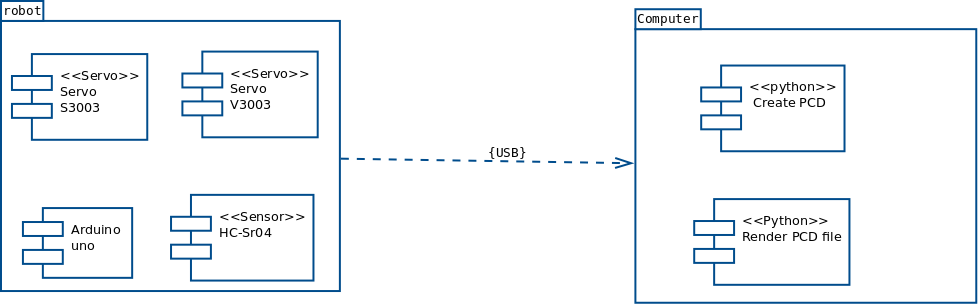
\includegraphics[scale=0.23]{deployment_digaram.png}
\end{figure}

\end{frame}


\section{Conclusion}
\begin{frame}{Conclusion}
\begin{itemize}
    \item Our project is to implement a two joint robot with an ultrasonic sensor that visualizes its surroundings.
    \item During the progress of the project we were learnt a lot of concepts.
    \item These concepts mainly comes under hardware and software sections 
    
\end{itemize}
\end{frame}
\begin{frame}{Conclusion}
   \item Hardware part
   \begin{itemize}
       \item[1)]3-D design and modelling
       \item[2)]Controlling of servo 
       \item[3)]Operations using the arduino
   \end{itemize}
\end{frame}
\begin{frame}{Conclusion}
    \begin{itemize}
        \item Software part
        \begin{itemize}
            \item[1)]Concept of point cloud and mapping the surroundings
            \item[2)]Generating the pcd file for visualization
        \end{itemize}
    \end{itemize}
\end{frame}





\end{document} 
